\documentclass[tikz,border=8pt]{standalone}
\usepackage{fontenc}
\usepackage{amsmath,amssymb}
\usetikzlibrary{shapes.geometric, shapes.misc, arrows.meta, positioning, fit, backgrounds, calc}

\newcommand{\nhdr}[1]{\textbf{#1}}
\newcommand{\nsub}[1]{{\footnotesize\itshape\color{black!55}#1}}

\begin{document}
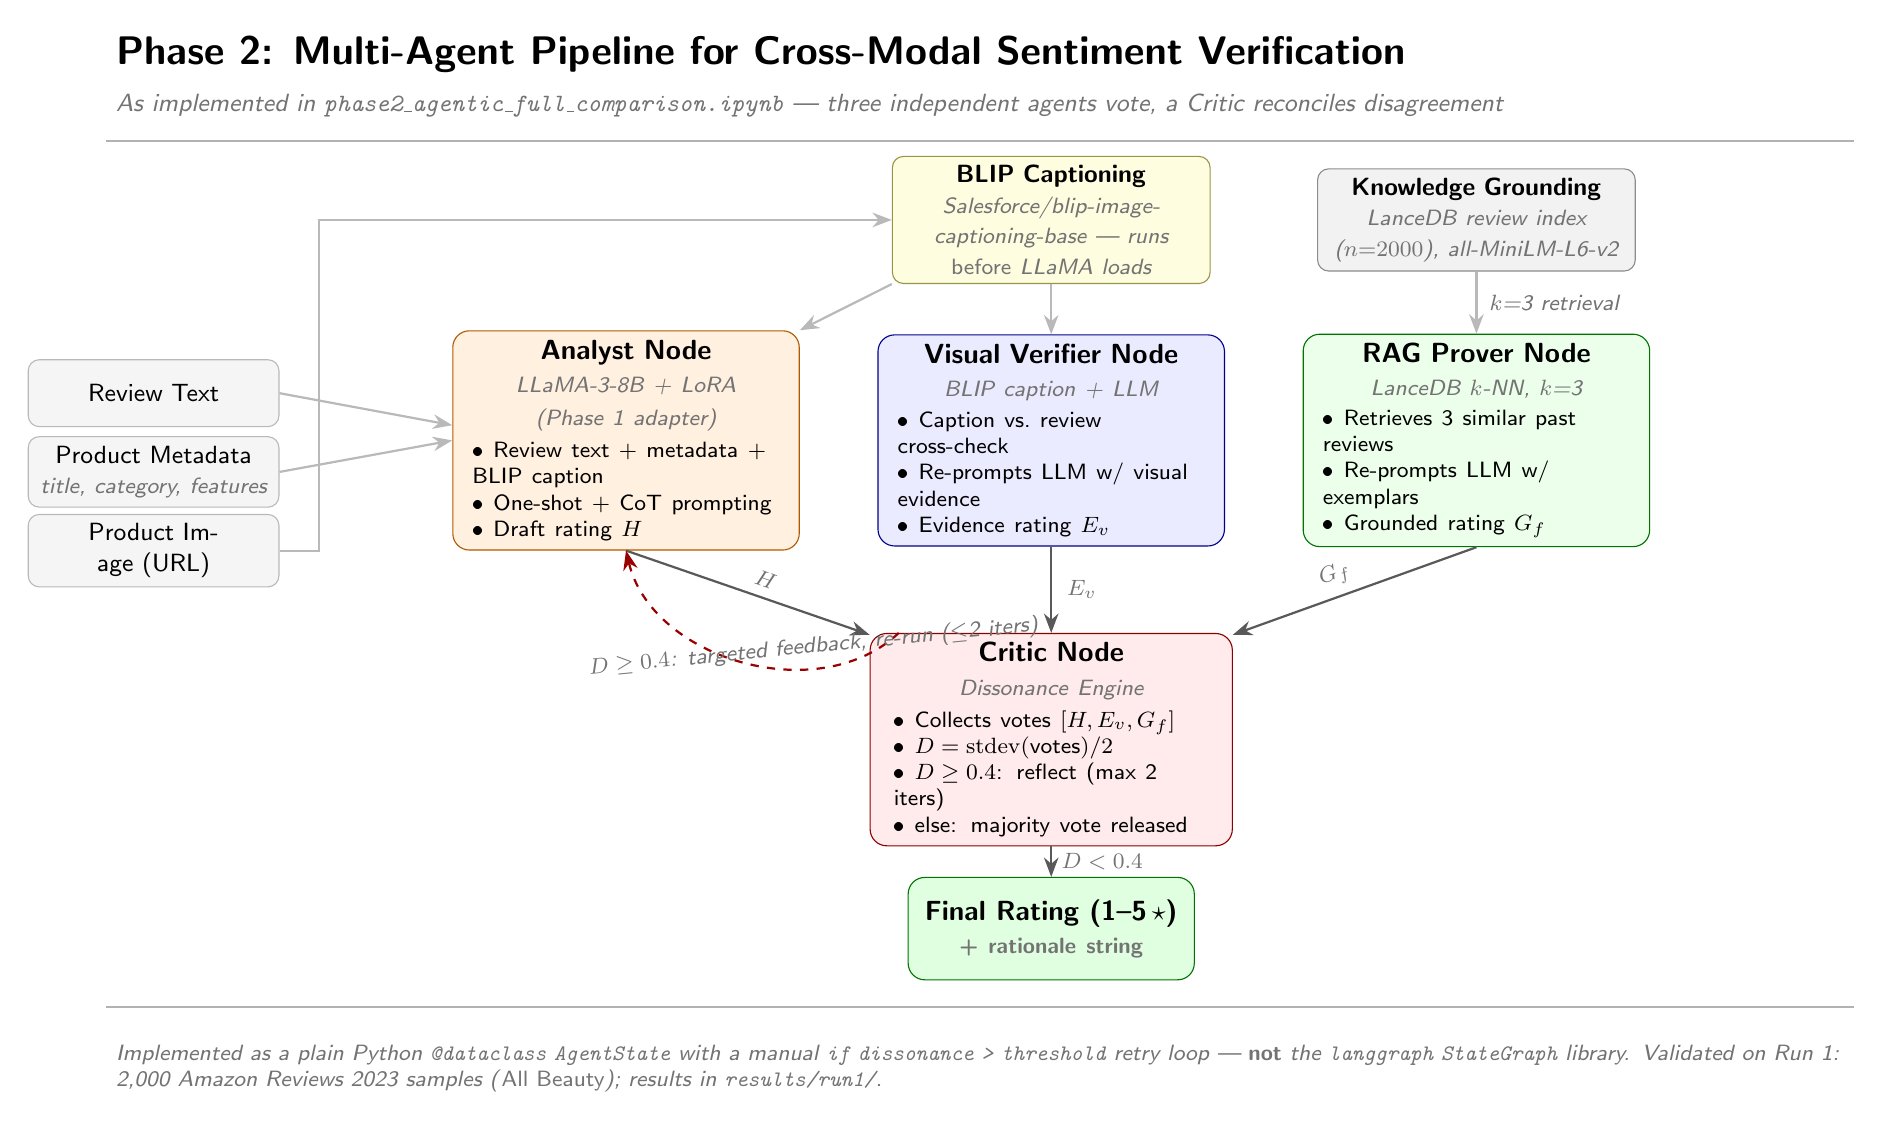
\begin{tikzpicture}[
  font=\sffamily,
  title/.style     = {font=\sffamily\bfseries\Large},
  subtitle/.style  = {font=\sffamily\itshape\small, text=black!55},
  inp/.style       = {rectangle, rounded corners=4pt, draw=gray!55, fill=gray!8,
                      minimum width=3.1cm, minimum height=0.85cm,
                      font=\sffamily\small, align=center, text width=2.95cm},
  resource/.style  = {rectangle, rounded corners=4pt, draw=black!45, fill=black!5,
                      minimum width=4.0cm, minimum height=1.1cm,
                      font=\sffamily\small, align=center, text width=3.8cm},
  analyst/.style   = {rectangle, rounded corners=6pt, draw=orange!70!black, fill=orange!12,
                      minimum width=4.4cm, minimum height=1.9cm,
                      font=\sffamily, align=center, text width=4.1cm},
  visual/.style    = {rectangle, rounded corners=6pt, draw=blue!55!black, fill=blue!8,
                      minimum width=4.4cm, minimum height=1.9cm,
                      font=\sffamily, align=center, text width=4.1cm},
  rag/.style       = {rectangle, rounded corners=6pt, draw=green!45!black, fill=green!8,
                      minimum width=4.4cm, minimum height=1.9cm,
                      font=\sffamily, align=center, text width=4.1cm},
  critic/.style    = {rectangle, rounded corners=6pt, draw=red!55!black, fill=red!8,
                      minimum width=4.6cm, minimum height=2.1cm,
                      font=\sffamily, align=center, text width=4.3cm},
  outbox/.style    = {rectangle, rounded corners=6pt, draw=green!45!black, fill=green!12,
                      minimum width=3.6cm, minimum height=1.3cm,
                      font=\sffamily\bfseries, align=center, text width=3.4cm},
  arr/.style       = {-{Stealth[length=7pt]}, thick, black!65},
  rarr/.style      = {-{Stealth[length=7pt]}, thick, red!60!black, dashed},
  garr/.style      = {-{Stealth[length=7pt]}, thick, gray!55},
  lbl/.style       = {font=\sffamily\footnotesize\itshape, text=black!55},
]

%% ══════════════════════════════════════════ Title ══════════════════════════════════════════
\node[title, anchor=west] (ttl) at (-5.6, 11.4) {Phase 2: Multi-Agent Pipeline for Cross-Modal Sentiment Verification};
\node[subtitle, anchor=west] (sub) at (-5.6, 10.75) {As implemented in \texttt{phase2\_agentic\_full\_comparison.ipynb} --- three independent agents vote, a Critic reconciles disagreement};
\draw[black!30, thick] (-5.6, 10.3) -- (16.6, 10.3);

%% ══════════════════════════════════════════ Resource row ══════════════════════════════════
\node[resource, fill=yellow!12, draw=yellow!55!black] (blip) at (6.4, 9.3) {
  \nhdr{BLIP Captioning}\\
  \nsub{Salesforce/blip-image-captioning-base --- runs \emph{before} LLaMA loads}
};
\node[resource] (kdb) at (11.8, 9.3) {
  \nhdr{Knowledge Grounding}\\
  \nsub{LanceDB review index ($n{=}2000$), all-MiniLM-L6-v2}
};

%% ══════════════════════════════════════════ Agent row ═════════════════════════════════════
\node[analyst] (analyst) at (1.0, 6.5) {
  \nhdr{Analyst Node}\\
  \nsub{LLaMA-3-8B + LoRA (Phase 1 adapter)}\\[3pt]
  \begin{minipage}{3.9cm}\raggedright\footnotesize
  \textbullet\ Review text + metadata + BLIP caption\\
  \textbullet\ One-shot + CoT prompting\\
  \textbullet\ Draft rating $H$
  \end{minipage}
};
\node[visual] (visual) at (6.4, 6.5) {
  \nhdr{Visual Verifier Node}\\
  \nsub{BLIP caption + LLM}\\[3pt]
  \begin{minipage}{3.9cm}\raggedright\footnotesize
  \textbullet\ Caption vs.\ review cross-check\\
  \textbullet\ Re-prompts LLM w/ visual evidence\\
  \textbullet\ Evidence rating $E_v$
  \end{minipage}
};
\node[rag] (rag) at (11.8, 6.5) {
  \nhdr{RAG Prover Node}\\
  \nsub{LanceDB $k$-NN, $k$=3}\\[3pt]
  \begin{minipage}{3.9cm}\raggedright\footnotesize
  \textbullet\ Retrieves 3 similar past reviews\\
  \textbullet\ Re-prompts LLM w/ exemplars\\
  \textbullet\ Grounded rating $G_f$
  \end{minipage}
};

%% ══════════════════════════════════════════ Critic + output ═══════════════════════════════
\node[critic] (critic) at (6.4, 2.7) {
  \nhdr{Critic Node}\\
  \nsub{Dissonance Engine}\\[3pt]
  \begin{minipage}{4.0cm}\raggedright\footnotesize
  \textbullet\ Collects votes $[H, E_v, G_f]$\\
  \textbullet\ $D = \mathrm{stdev}(\text{votes}) / 2$\\
  \textbullet\ $D \geq 0.4$: reflect (max 2 iters)\\
  \textbullet\ else: majority vote released
  \end{minipage}
};
\node[outbox] (final) at (6.4, 0.3) {Final Rating (1--5\,$\star$)\\\nsub{+ rationale string}};

%% ══════════════════════════════════════════ Inputs (left column) ══════════════════════════
\node[inp] (rev)  at (-5.0, 7.1) {Review Text};
\node[inp] (meta) at (-5.0, 6.1) {Product Metadata\\\nsub{title, category, features}};
\node[inp] (img)  at (-5.0, 5.1) {Product Image (URL)};

%% ══════════════════════════════════════════ Input → Analyst ═══════════════════════════════
\draw[garr] (rev.east)  -- (analyst.175);
\draw[garr] (meta.east) -- (analyst.west);

%% ══════════════════════════════════════════ Image → BLIP → {Analyst, Visual Verifier} ═════
\draw[garr] (img.east) -- ++(0.5,0) |- (blip.west);
\draw[garr] (blip.south west) -- (analyst.north east);
\draw[garr] (blip.south) -- (visual.north);

%% ══════════════════════════════════════════ Knowledge grounding → RAG ═════════════════════
\draw[garr] (kdb.south) -- node[lbl, right, xshift=1pt]{$k$=3 retrieval} (rag.north);

%% ══════════════════════════════════════════ Three independent votes → Critic ══════════════
\draw[arr] (analyst.south) -- node[lbl, above, sloped, pos=0.55]{$H$} (critic.150);
\draw[arr] (visual.south)  -- node[lbl, right, xshift=2pt]{$E_v$} (critic.north);
\draw[arr] (rag.south)     -- node[lbl, above, sloped, pos=0.55]{$G_f$} (critic.30);

%% ══════════════════════════════════════════ Critic decision ═══════════════════════════════
\draw[arr] (critic.south) -- node[lbl, right]{$D < 0.4$} (final.north);
\draw[rarr] (critic.145) to[bend left=60] node[lbl, above, sloped, pos=0.28]{$D \geq 0.4$: targeted feedback, re-run ($\leq$2 iters)} (analyst.south);

%% ══════════════════════════════════════════ Footnote ══════════════════════════════════════
\draw[black!30, thick] (-5.6, -0.7) -- (16.6, -0.7);
\node[lbl, anchor=north west, text width=22.2cm, align=left] at (-5.6, -1.05)
 {Implemented as a plain Python \texttt{@dataclass AgentState} with a manual \texttt{if dissonance > threshold} retry loop --- \textbf{not} the \texttt{langgraph} \texttt{StateGraph} library. Validated on Run~1: 2{,}000 Amazon Reviews 2023 samples (\emph{All Beauty}); results in \texttt{results/run1/}.};

\end{tikzpicture}
\end{document}
